%%%%%%%%%%%%%%%%%%%%%%%%%%%%%%%%%%%%%%%%%
% Journal Article
% LaTeX Template
% Version 1.4 (15/5/16)
%
% This template has been downloaded from:
% http://www.LaTeXTemplates.com
%
% Original author:
% Frits Wenneker (http://www.howtotex.com) with extensive modifications by
% Vel (vel@LaTeXTemplates.com)
%
% License:
% CC BY-NC-SA 3.0 (http://creativecommons.org/licenses/by-nc-sa/3.0/)
%
%%%%%%%%%%%%%%%%%%%%%%%%%%%%%%%%%%%%%%%%%

%----------------------------------------------------------------------------------------
%	PACKAGES AND OTHER DOCUMENT CONFIGURATIONS
%----------------------------------------------------------------------------------------

\documentclass[twoside,twocolumn]{article}

\usepackage{blindtext} % Package to generate dummy text throughout this template 

\usepackage[sc]{mathpazo} % Use the Palatino font
\usepackage[T1]{fontenc} % Use 8-bit encoding that has 256 glyphs
\linespread{1.05} % Line spacing - Palatino needs more space between lines
\usepackage{microtype} % Slightly tweak font spacing for aesthetics

\usepackage[spanish, english]{babel} % Language hyphenation and typographical rules
\usepackage[utf8]{inputenc}

\usepackage[hmarginratio=1:1,top=32mm,columnsep=20pt]{geometry} % Document margins
\usepackage[hang, small,labelfont=bf,up,textfont=it,up]{caption} % Custom captions under/above floats in tables or figures
\usepackage{booktabs} % Horizontal rules in tables

\usepackage{lettrine} % The lettrine is the first enlarged letter at the beginning of the text

\usepackage{enumitem} % Customized lists
\setlist[itemize]{noitemsep} % Make itemize lists more compact

\usepackage{abstract} % Allows abstract customization
\renewcommand{\abstractnamefont}{\normalfont\bfseries} % Set the "Abstract" text to bold
\renewcommand{\abstracttextfont}{\normalfont\small\itshape} % Set the abstract itself to small italic text

\usepackage{titlesec} % Allows customization of titles
\renewcommand\thesection{\Roman{section}} % Roman numerals for the sections
\renewcommand\thesubsection{\roman{subsection}} % roman numerals for subsections
\titleformat{\section}[block]{\large\scshape\centering}{\thesection.}{1em}{} % Change the look of the section titles
\titleformat{\subsection}[block]{\large}{\thesubsection.}{1em}{} % Change the look of the section titles

\usepackage{fancyhdr} % Headers and footers
\pagestyle{fancy} % All pages have headers and footers
\fancyhead{} % Blank out the default header
\fancyfoot{} % Blank out the default footer
\fancyhead[C]{Golang $\bullet$ Aug 2019 $\bullet$ Vol. I, No. 1} % Custom header text
\fancyfoot[RO,LE]{\thepage} % Custom footer text

\usepackage{titling} % Customizing the title section

\usepackage{hyperref} % For hyperlinks in the PDF
\usepackage{graphicx}

%----------------------------------------------------------------------------------------
%	TITLE SECTION
%----------------------------------------------------------------------------------------

\setlength{\droptitle}{-4\baselineskip} % Move the title up

\pretitle{\begin{center}\Huge\bfseries} % Article title formatting
\posttitle{\end{center}} % Article title closing formatting
\title{Algoritmos de Inteligencia Artificial y Machine Learning en Go} % Article title
\author{%
\textsc{Salvador E. Venegas-Andraca} \\[1ex] % Your name
\normalsize Tecnológico de Monterrey, Escuela de Ingeniería y Ciencias \\ % Your institution
\normalsize \href{mailto:salvador.venegas-andraca@keble.oxon.org}{salvador.venegas-andraca@keble.oxon.org} % Your email address
\and % Uncomment if 2 authors are required, duplicate these 4 lines if more
\textsc{José M. Miranda Villagrán} \\[1ex] % Second author's name
\normalsize Instituto Tecnológigo de Veracruz \\ % Second author's institution
\normalsize \href{mailto:mirandav@itver.edu.mx}{mirandav@itver.edu.mx} % Second author's email address
\and % Uncomment if 2 authors are required, duplicate these 4 lines if more
\textsc{Gabriel Acosta} \\[1ex] % Second author's name
\normalsize Instituto Politécnico Nacional \\ % Second author's institution
\normalsize \href{mailto:algo@algo.com}{algo@algo.com} % Second author's email address
}
\date{\today} % Leave empty to omit a date
\renewcommand{\maketitlehookd}{%
\begin{abstract}
\noindent 
En este articulo se explica la etapa actual del hardware y software de la computadora y por qué necesitamos un nuevo lenguaje como Go. 
\end{abstract}
}

%----------------------------------------------------------------------------------------

\begin{document}

% Print the title
\maketitle

%----------------------------------------------------------------------------------------
%	ARTICLE CONTENTS
%----------------------------------------------------------------------------------------

\section{Introducción}

\lettrine[nindent=0em,lines=3]{E} n los últimos años, ha surgido un nuevo lenguaje de programación: Go o GoLang. Se presentó el 10 de noviembre de 2009 como un nuevo lenguaje de programación con tiempos de compilación muy rápido. Las excelentes herramientas de Go, el elegante modelo de concurrencia y el enfoque único de la orientación a objetos ha cautivado la atención de los desarrolladores tanto de los lenguajes compilados como de los scripts.

\subsection{Limitaciones de hardware}

El primer procesador Pentium 4 con velocidad de reloj de 3.0 GHz\footnote{\url{ http://www.informit.com/articles/article.aspx?p=339073}} fue presentado en 2004 por Intel. Actualmente los equipos comerciales tienen una velocidad de reloj de 2.30GHz. Entonces, casi en una década, no hay demasiada ganancia en el poder de procesamiento en bruto. Se puede ver la comparación de aumento de potencia de procesamiento con respecto al tiempo en la figura \ref{fig1}.

\begin{figure}[htbp]
	\centerline{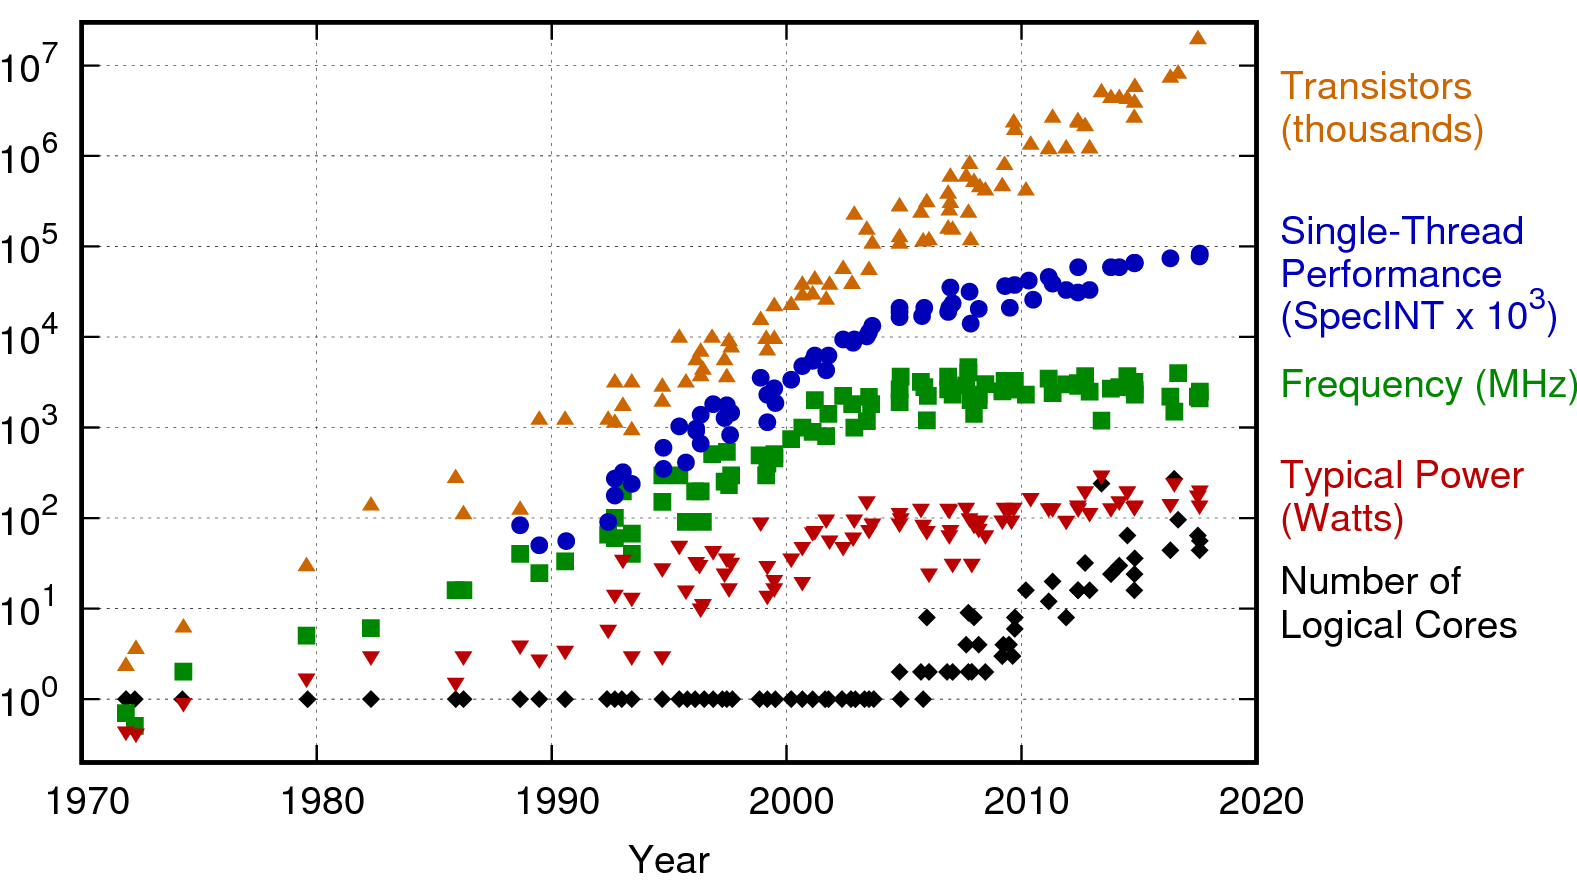
\includegraphics[scale=0.22]{img/42-years-processor-trend.png}}
	\caption{\textit{42 años de tendencias de microprocesadores.}}
	\label{fig1}
\end{figure}

\noindent
En el gráfico anterior puede ver que el rendimiento de un solo hilo y la frecuencia del procesador se mantuvieron estables durante casi una década. Agregar más transistores no es la solución. Esto se debe a que a menor escala comienzan a surgir algunas propiedades cuánticas y porque en realidad cuesta más poner más transistores.

Entonces, para la solución del problema anterior los fabricantes comenzaron a agregar más núcleos al procesador, también introdujeron hyper-threading y se agregó más caché al procesador para aumentar el rendimiento.

Pero las soluciones anteriores también tienen sus propias limitaciones. No podemos agregar más caché al procesador para aumentar el rendimiento ya que el caché tiene límites físicos: cuanto más grande es el caché, más lento se vuelve\footnote{\url{https://www.researchgate.net/post/Why_is_the_capacity_of_of_cache_memory_so_limited}}. Agregar más núcleos al procesador también tiene su costo. Estos procesadores multinúcleo pueden ejecutar varios procesos simultáneamente y eso brinda concurrencia.

Por lo tanto, si no podemos confiar en las mejoras de hardware, el único camino a seguir es un software más eficiente para aumentar el rendimiento. Pero lamentablemente, los lenguajes de programación modernos no son muy eficientes.

%------------------------------------------------

\subsection{¿Por qué Go?}

\begin{quote}

	\small "Go will be the server language of the future." - Tobias Lütke\footnote{\url{https://en.wikipedia.org/wiki/Tobias_Lütke}}, Shopify

\end{quote}

\noindent
Para evaluar el lenguaje Go como una solución para el desarrollo web moderno, hay que ver las tendencias y considerar que debería proporcionar "el lenguaje servidor del futuro".\footnote{\url{https://nathany.com/why-go/}}

Los fabricantes de hardware están agregando más y más núcleos a los procesadores para aumentar el rendimiento. Todos los centros de datos funcionan con esos procesadores. Además, las aplicaciones actuales utilizan múltiples microservicios para mantener conexiones de bases de datos, colas de mensajes y mantener cachés. Por lo tanto, el software que se desarrolla y los lenguajes de programación deben admitir la concurrencia fácilmente y deben ser escalables con un mayor número de núcleos.

Pero, la mayoría de los lenguajes de programación modernos (como Java, Python, etc.) son del entorno de subproceso único de los años 90. La mayoría de esos lenguajes de programación admite subprocesos múltiples. Pero el verdadero problema viene con la ejecución concurrente, el bloqueo de subprocesos, las condiciones de carrera y los puntos muertos. Esas cosas hacen que sea difícil crear una aplicación de subprocesos múltiples en esos lenguajes.




%------------------------------------------------

\section{Methods}

Maecenas sed ultricies felis. Sed imperdiet dictum arcu a egestas. 
\begin{itemize}
\item Donec dolor arcu, rutrum id molestie in, viverra sed diam
\item Curabitur feugiat
\item turpis sed auctor facilisis
\item arcu eros accumsan lorem, at posuere mi diam sit amet tortor
\item Fusce fermentum, mi sit amet euismod rutrum
\item sem lorem molestie diam, iaculis aliquet sapien tortor non nisi
\item Pellentesque bibendum pretium aliquet
\end{itemize}
\blindtext % Dummy text

Text requiring further explanation\footnote{Example footnote}.

%------------------------------------------------

\section{Results}

\begin{table}
\caption{Example table}
\centering
\begin{tabular}{llr}
\toprule
\multicolumn{2}{c}{Name} \\
\cmidrule(r){1-2}
First name & Last Name & Grade \\
\midrule
John & Doe & $7.5$ \\
Richard & Miles & $2$ \\
\bottomrule
\end{tabular}
\end{table}

\blindtext % Dummy text

\begin{equation}
\label{eq:emc}
e = mc^2
\end{equation}

\blindtext % Dummy text

%------------------------------------------------

\section{Discussion}

\subsection{Subsection One}

A statement requiring citation \cite{Figueredo:2009dg}.
\blindtext % Dummy text

\subsection{Subsection Two}

\blindtext % Dummy text

%----------------------------------------------------------------------------------------
%	REFERENCE LIST
%----------------------------------------------------------------------------------------

\begin{thebibliography}{99} % Bibliography - this is intentionally simple in this template

\bibitem[Figueredo and Wolf, 2009]{Figueredo:2009dg}
Figueredo, A.~J. and Wolf, P. S.~A. (2009).
\newblock Assortative pairing and life history strategy - a cross-cultural
  study.
\newblock {\em Human Nature}, 20:317--330.
 
\end{thebibliography}

%----------------------------------------------------------------------------------------

\end{document}
